\pdfoutput=1
% In particular, the hyperref package requires pdfLaTeX in order to break URLs across lines.

\documentclass[11pt]{article}

% Remove the "review" option to generate the final version.
\usepackage{ACL2023}
\usepackage{graphicx}
\usepackage{lipsum} % For generating dummy text
\usepackage{wrapfig} % For wrapping text around figures

\usepackage{tikz}
\usepackage{graphicx} % for including images
\usepackage[margin=0pt, paperwidth=\textwidth, paperheight=\textheight, showframe]{geometry} % Adjust margins and show frame for demonstration
\usepackage{array}
\usepackage{adjustbox}
\usepackage{tabularx}

% Standard package includes
\usepackage{times}
\usepackage{latexsym}

% For proper rendering and hyphenation of words containing Latin characters (including in bib files)
\usepackage[T1]{fontenc}
% For Vietnamese characters
% \usepackage[T5]{fontenc}
% See https://www.latex-project.org/help/documentation/encguide.pdf for other character sets

% This assumes your files are encoded as UTF8
\usepackage[utf8]{inputenc}

% This is not strictly necessary, and may be commented out.
% However, it will improve the layout of the manuscript,
% and will typically save some space.
\usepackage{microtype}

% This is also not strictly necessary, and may be commented out.
% However, it will improve the aesthetics of text in
% the typewriter font.
\usepackage{inconsolata}

\usepackage{float}

% If the title and author information does not fit in the area allocated, uncomment the following
%
%\setlength\titlebox{<dim>}
%
% and set <dim> to something 5cm or larger.

\title{Final Report: Options Algorithm }


\author{Saumya Bajaj, Abinav Chari, Mark Rodrigues, Riya Bhadani, Daniel Wu}



\begin{document}

\maketitle
\begin{abstract}
We continued the project from last semester into this semester, addressing not only the issues but also expanding the scope of our model.

One of our primary objectives was to experiment with more data. Furthermore, we wanted to work on feature reduction as many of our features had very high correlations.

Additionally, we would include better features such as the stock price derivative estimation, Bjerksund-Stensland Model inverted volatility, and Trinomial Option Pricing to help us increase the accuracy and precision of our model.

This semester the team focused on calculating implied volatility for the binomial options pricing model. While Implied Volatility was calculated, due to challenges inherent to the Bjerksund-Stensland Model, the resulting volatility was inaccurate.

As such, the team decided that in order to maintain the existing integrity and accuracy of the model, Trinomial Option Pricing would not be calculated.

In addition to feature engineering, we also aimed to work with new models such as the Garch Model, RNN and LSTM, and CNNs. 

Furthermore, we explored comparing latency with Random Forest, as Random Forests and Boosting Models, which were the models we previously experimented with, have limitations that may be overcome by other models.

Finally, the ultimate goal for this semester was to create an online learning model by using a continuous stream of real-time data to update model parameters. 

We then would experiment with online RF methods and RNNs trained with streamed data, finally comparing speed and performance with the offline versions.

\end{abstract}

\section{Introduction}

Last semester, the team’s goal was to create a classification model for options that determined  the ideal exit time of an at-the-money short straddle position as per market conditions. 

We got our data by simulation the stop-loss variation and the fixed stop-loss variation on options data from the past two years pulled from Polygon. The team trained Random Forest, XGBoost, CatBoost, and LightGBM models using the data collected. 

The accuracy rate of the models hovered at about 60 percent and with the exception of CatBoost, the models produced similar max profits in comparison to the actual data. 

In order to improve the accuracy and usefulness of the models and build a more robust strategy, the team is focused on improving feature selection this semester by doing feature reduction and selecting  better features. 

Last semester there were too many features and many of the features were highly correlated leading to high inefficiency. This is where most of the work has been done thus far. 

The team focused on understanding how the Greek Indicators, Bjerksund-Stensland model, and trinomial option pricing could be implemented as features. 

The team attempted to implement implied volatility but eventually decided against using it in the model as data collection proved challenging. 

As such, the plan to calculate the Trinomial Option Pricing Model was scrapped to maintain the accuracy of the model.

\section{Greek Indicators}
 The Greeks refer to a set of metrics used in options trading to measure the sensitivity of an option's price to various factors. They include delta and gamma. 

Delta measures how much an option's price changes compared to a 1-dollar change in the underlying asset's price. It reflects the option's price sensitivity to movements in the underlying.

Gamma measures the rate of change of delta with respect to changes in the underlying price. It indicates how much delta itself will change as the asset price moves.

We decided to include such metrics as part of our features to investigate if they can improve the accuracy of our prediction. We calculated Delta to be how much the straddle exit changes compared to a 1-dollar change of the SPX. 

Similarly, gamma was calculated as the rate of change of delta with respect to changes in the underlying price. In order to obtain a function of the Straddle Exit value and the SPX close, a cubic spline was used (Figure 1).

% \begin{center}
%     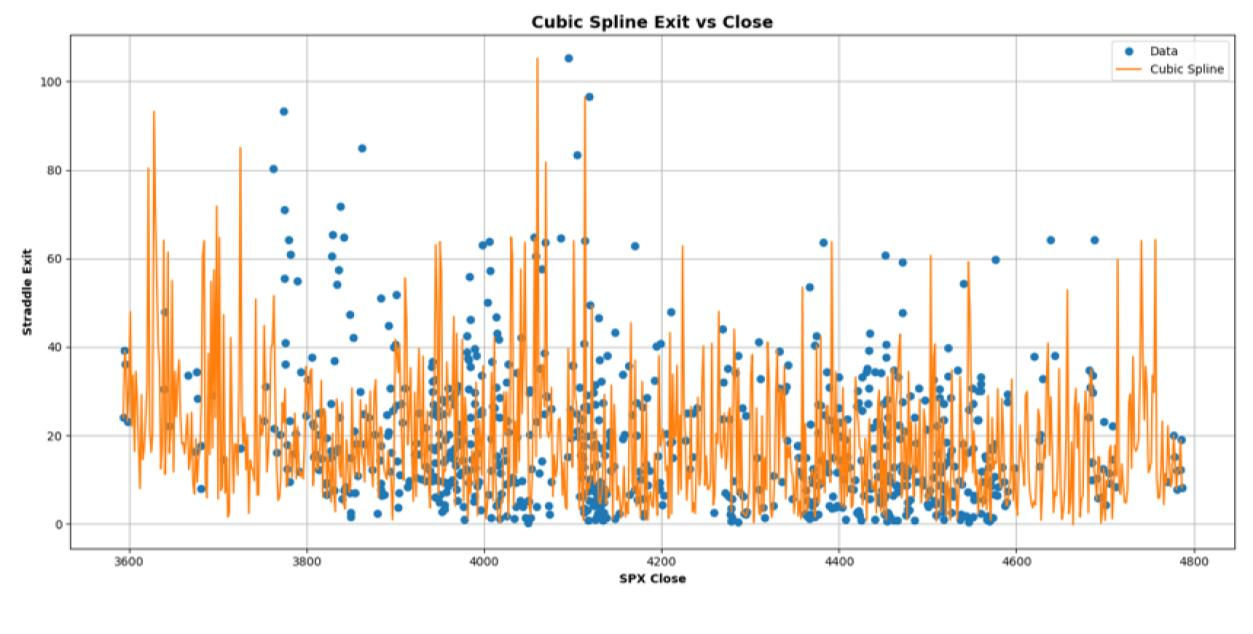
\includegraphics[width=1\textwidth]{pic1.jpg}
%     \captionof{figure}{The spline function fitted to Straddle exit vs SPX close}
%     \label{fig:example}
% \end{center}



\begin{figure*}[!t]
    \centering
    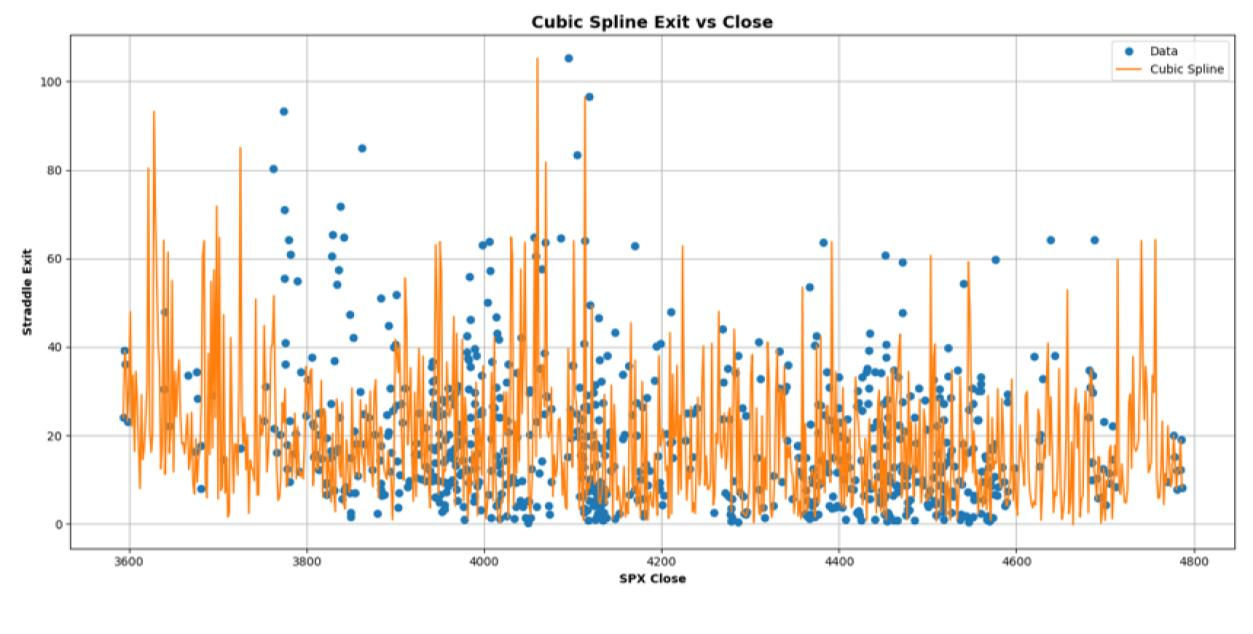
\includegraphics[width=\textwidth]{pic1.jpg} % Replace with the path to your image
    \caption{The spline function fitted to Straddle exit vs SPX close}
\end{figure*}


The derivatives were calculated accordingly and added as features to assist in the prediction (Figure 2 and 3).


% \begin{figure*}[!t]
%     \centering
%     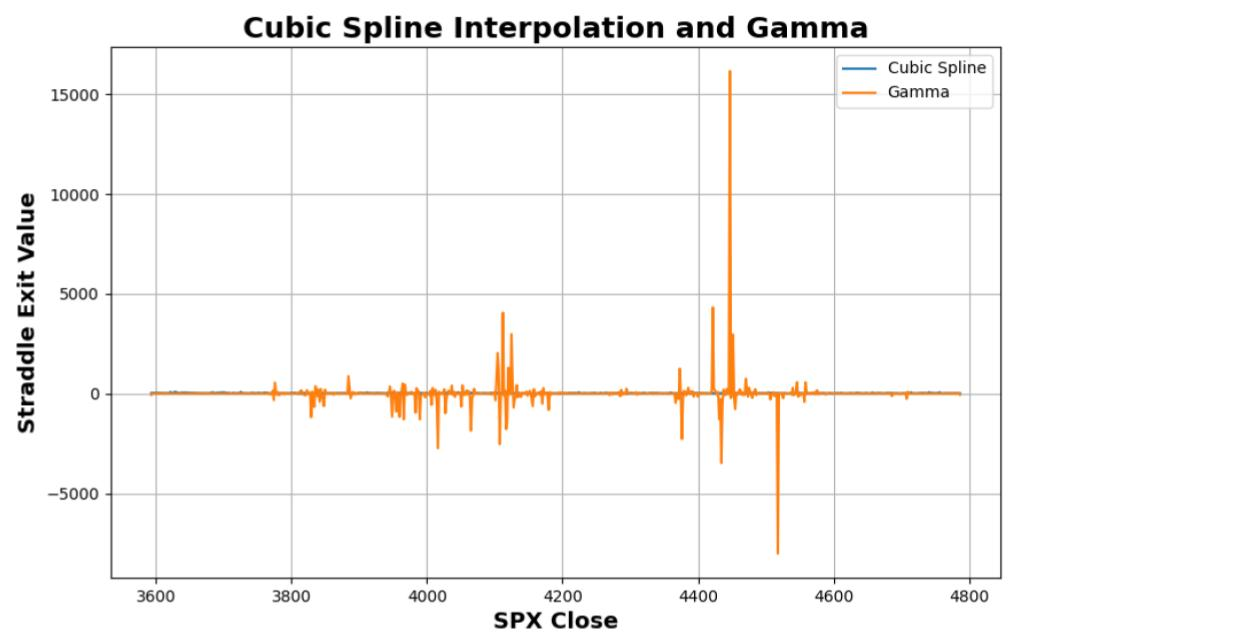
\includegraphics[width=\textwidth]{pic2.jpg} % Replace with the path to your image
%     \caption{1st Derivative of the Spline Function}
% \end{figure*}


\begin{figure}[H]
    \centering
    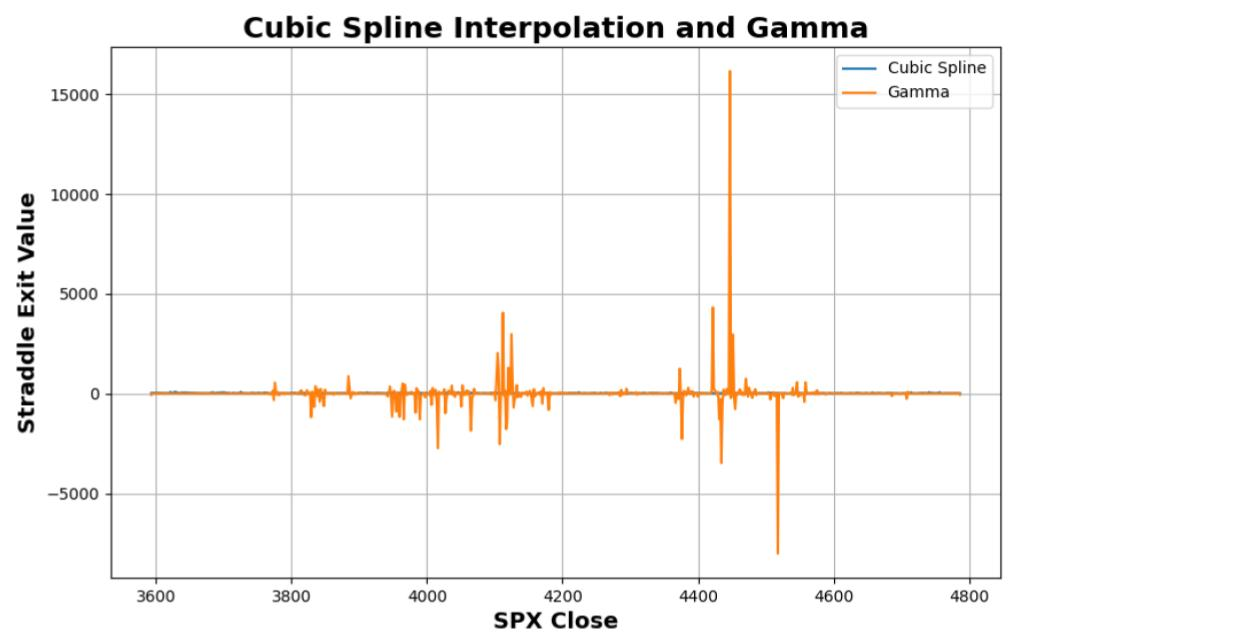
\includegraphics[width=0.6\textwidth]{pic2.jpg} % Replace 'example-image' with the filename of your image
    \caption{1st Derivative of the Spline Function}
    \label{fig:example}
\end{figure}


\begin{figure}[H]
    \centering
    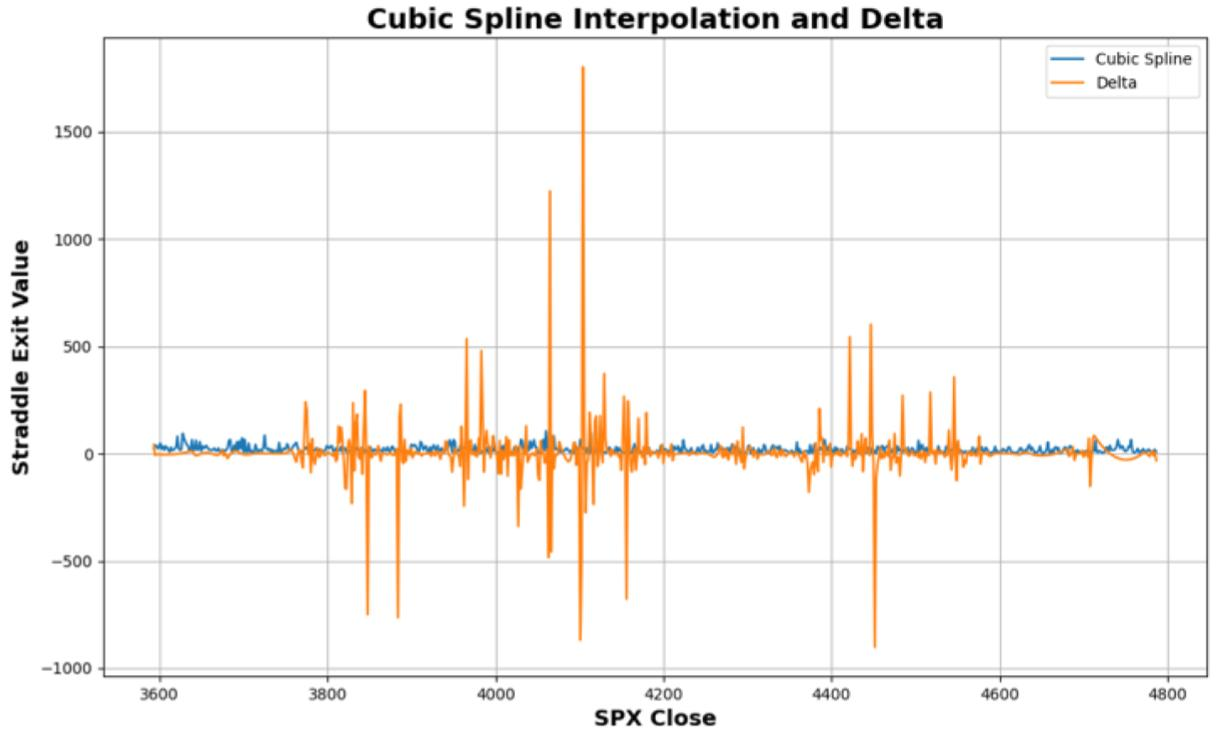
\includegraphics[width=0.5\textwidth]{pic3 (1).jpg} % Replace 'example-image' with the filename of your image
     \caption{2nd Derivative of the Spline Function}
    \label{fig:example}
\end{figure}

% \begin{figure}[H]
%     \centering
%     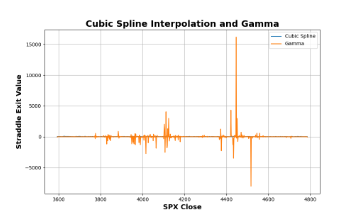
\includegraphics[width=0.5\textwidth]{graph2.png} % Replace 'example-image' with the filename of your image
%     \caption{2nd Derivative of the Spline Function}
%     \label{fig:example}
% \end{figure}

The features were added to the data set and we evaluated the effectiveness of these features on accuracy by running our random forest classifier (one of our most successful models) on the new data set with the added features. The accuracy of the RFC increased by about 2\% from 66.8\% to 69\%. 

In addition, when testing for feature importance, the new indicators made it to the top 20 features among a list of over 115 features. The delta was ranked as the 6\textsuperscript{th} most important feature while the gamma was ranked as the 16\textsuperscript{th} most important feature. 

Despite this success, after performing a hypothesis test on the addition of these new features, the results of the test were insignificant. This insignificance is likely due to the delta and gamma being correlated with other features. 

So while they may not be individually significant, these two indicators are jointly significant with other features in the data set. 

\begin{figure}[H]
    \centering
    \includegraphics[width=.5\textwidth]{Screenshot 2024-04-20 at 2.02.35 PM} % Replace 'example-image' with the filename of your image
    \caption{Classification Report for new features}
    \label{fig:example}
\end{figure}


\section{Implied Volatility}
The  researchers attempted to implement implied volatility in order to use the binomial option pricing model as a feature. 

Initially, the researchers planned to base their computational calculation of implied volatility using code calculating the inversion of the Black-Scholes Formula, previously coded by a team member, as discussed in the midterm report. 

This was not possible, however, as the team later learned. Unlike the Black-Scholes Equation, which is closed-form, the Bjerksund-Stensland model is open-form. Therefore it is not possible to rearrange the Bjerksund-Stensland formula to solve for implied volatility. 

Instead, an iterative method must be implemented. The researcher used the Newton-Raphson Method. A challenge with this method was it involved determining an initial estimated implied volatility that was refined through each iteration. 

If the estimate is far from the truth, then the model may oscillate, requiring more iterations or fail to diverge completely. 0.2 was used as the initial estimate. This was based on the 0.15 average implied volatility of options. 

The researcher chose to use a slightly higher estimate as the options they were examining were backed by technology stocks that are typically more volatile. In the future, a more informed estimated volatility should be calculated. 

A challenge with relying on a single estimate for all the options to researchers was testing was the historical implied volatilities of the options vary greatly, with AAPL being at \~28.6\% and NVDA at \~47.5\%. 

Alternative iterative methods should also be considered in order to find the best calculation and account for mischosen initial estimates and the variability between options within the same section. The bisection method may be useful as it considers two initial estimates, one higher and one lower.


\subsection{Results}

\begin{table}[H]
    \centering
    \begin{adjustbox}{width=0.5\textwidth}
    \begin{tabularx}{\linewidth}{|X|X|X|}
        \hline
        \textbf{Option} & \textbf{Average Calculated Implied Volatility (\%)} & \textbf{Average Historical Implied Volatility (\%)} \\
        \hline
        AAPL & 5.60 & 25.60 \\
        \hline
        AMZN & 4.99 & 31.03 \\
        \hline
        GOOG & 4.84 & 36.98 \\
        \hline
        MSFT & 5.74 & 31.17 \\
        \hline        
        META & 9.07 & 81.66 \\
        \hline       
        NVDA & 34.17 & 47.50 \\
        
        \hline
    \end{tabularx}
    \end{adjustbox}
    \caption{Comparison of Calculated and Historical Volatility}
    \label{tab:volatility_comparison}
\end{table}
Initially, it appeared that the computational results were off by a factor of 6; however, the results of META and NVDA prove this to be otherwise. 

It is unclear why the result of NVDA is particularly high, especially since its historical implied volatility is not drastically different than the others. 

\subsection{Challenges and Conclusions}
A major issue the team had with calculating implied volatility was finding the data. The calculation required dividend yield, expiration date, strike price, and historical prices. 

The team already had access to the option price from last semester which they had pulled from Polygon. The team was also able to find all options contracts for the desired companies on Polygon; however, due to how Polygon data is formatted, the team could only access contracts with expiration dates of that day. 

In order to access contracts with other expiration dates, they would have needed to iterate through each date for at least the next three years, which would have been inefficient and impractical. 

The team also briefly considered the finance API as an alternate data source. The API provides access to a list of all the options contracts of a company and a list of the expiration dates. 

However, the lists were not linked, making it impossible to get one from the other. As a quick workaround, the researcher hard-coded the information of contracts that expire in three years for each company to get a baseline value.

Ultimately the team decided not to use implied volatility as a reliable model cannot be created within the constructs of the data available.

\section{Trinomial Option Pricing Model}

The team also investigated using the Trinomial Option Pricing model versus the Binomial Option Pricing model. 

In a binomial tree, the underlying price of the model must either increase or decrease at each node, with no provision for holding steady values. However, in a trinomial tree, the underlying price of the model can take on one of three values: higher, steady, or lower. Additionally, the Trinomial Tree typically recombines whenever the price decreases, meaning that at each step where the price decreases, there are multiple paths leading to the same price level.

This difference in structure between binomial and trinomial trees allows for a more nuanced representation of price movements in the trinomial model. By accommodating steady prices and recombining paths, the trinomial approach provides a more flexible and potentially more accurate representation of market dynamics.

An advantage of the binomial model is that it doesn't converge as quickly as the trinomial model, even by the fifth point. However, the trinomial model ultimately proves to be a better fit because it seamlessly integrates with our current program. It simplifies the calculations by considering only lower, higher, or steady price movements, aligning well with our existing framework.

While the binomial model may offer slower convergence, the trinomial model's compatibility with our system outweighs this consideration. Its straightforward approach to pricing movements allows for easier integration and maintenance within our program, streamlining our processes and ensuring accuracy in our calculations.

Furthermore under the trinomial model, for Vanilla Options, options in which the owner has the right but not the obligation to buy or sell the underlying asset at a predetermined price for a premium, the increasing number of iterations is often made irrelevant due to rapid convergence; however, the inclusion of the holding steady option is important. 

The process is represented mathematically as follows, where $u$ is up, $d$ is down, and $m$ is stable.
\begin{figure}[H]
    \centering
    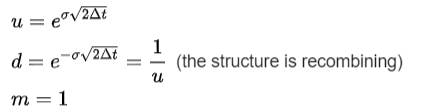
\includegraphics[width=0.5\textwidth]{eq1.png} 
    \caption{Equations for Trinomial Model}
    \label{fig:example}
\end{figure}

\begin{figure}[H]
    \centering
    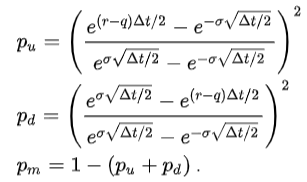
\includegraphics[width=0.5\textwidth]{eq2.png} 
    \caption{Probabilities for Trinomial Model}
    \label{fig:example}
\end{figure}
One issue is that the volatility, $\sigma$, is needed, so the team decided to use the volatility calculations from inverting the Bjerksund-Stensland Equation.

Ultimately, the volatility calculations from the Bjreksund-Stensland Equation were found to be inaccurate. To maintain the level of accuracy the team had achieved, they decided that the issue of using the Trinomial Option Pricing via inverted volatility was too large to overcome. 

This decision stemmed from a recognition that relying on the inverted volatility method posed significant challenges that could compromise the accuracy of their calculations. Despite efforts to mitigate these challenges, the team concluded that the inherent inaccuracies outweighed any potential benefits, prompting them to seek alternative approaches for volatility calculations.

As a result, the Trinomial Option Pricing Model results were excluded from the model. This decision was driven by concerns that incorporating them could either compromise the existing accuracy of the model or fail to produce a statistically significant change in accuracy.

The team opted for caution, prioritizing the preservation of the model's reliability. They determined that the potential impact on accuracy, whether positive or negative, did not justify the inclusion of the Trinomial Option Pricing Model results.

\section{LSTM Network}
The team also explored the implementation of an LSTM network for classifying whether or not to exit. We started with a combination of 25 features, including those we had previously selected for the random forest classifier, such as the RSI, volume, and super-trend of top performers like AAPL, AMZN, GOOG, NVDA, etc.

Initially, these features served as inputs for the LSTM model, which we aimed to train for decision-making in exiting trades. By leveraging this network, we sought to improve our trading strategy's accuracy and responsiveness to market conditions, particularly for high-performing stocks.

For simplicity, we set the hidden size to 1 and the learning rate to 0.001, using an Adam optimizer and a binary cross-entropy loss function. Our focus was on experimenting with the look-back window of our LSTM network, testing values of 5, 10, and 20.

By varying the look-back window size, we aimed to understand how different historical data lengths might impact the network's ability to make accurate exit decisions. This experimentation allowed us to fine-tune the model for optimal performance, ensuring it effectively captured relevant patterns and trends in the stock data.

After training for 100 epochs, all three of the LSTM classifiers had training loss curves that converged at values between 0.65 to 0.7. The LSTM with a look-back of 20 performed the best overall, with the lowest validation loss convergence around 0.65 and the highest AUC ROC score of 0.67. 

This LSTM also had the highest test accuracy of 68.9 percent. However, it also had the longest training time of 11.93 seconds. 

The LSTM with a look-back window of 5 had the highest validation loss convergence around 0.71 and even gradually increased towards the end, indicating possible overfitting. This model also had AUC ROC score of 0.49, performing worse than random guessing. With a training time of 4.86 seconds, it resulted in a lower test accuracy of 60.4 percent. 

The LSTM with a look-back of 10 had a performance roughly in the middle as expected. The validation loss converged at around 0.69, it had an AUC ROC score of 0.63, and surprisingly also had the same accuracy of 60.4 percent. 

This indicates that increasing the look-back window can increase the performance of the algorithm at a cost of higher training time, which makes sense because increasing the look-back window increases the amount of data we are feeding into the LSTM.

From the training and validation loss curves, it's evident that LSTMs, regardless of the look-back window size, tend to underfit the data. The training and validation loss curves depicted in Figure 6 and Figure 7 all converge at relatively high values of 0.6 and above. This convergence suggests that the model struggles to capture the underlying structure of the data adequately.

Another sign of underfitting is that all three LSTMs chose to stay in most situations and rarely decided to exit. Figure 10, Figure 11, and Figure 12 all show exit predictions only in the single digits, with Figure 11 showing no predictions for exiting at all compared to the 30 to 40 predictions made for staying. This could be because the data that we trained on has more instances of staying rather than exiting. The underfitting problem could be made less prevalent by training the LSTM with more examples of exiting.

The consistently high loss values indicate that the LSTM models are unable to effectively learn from the training data, resulting in suboptimal performance. This underfitting phenomenon implies that the models are not complex enough to capture the intricate patterns present in the stock data, highlighting the need for further exploration and refinement of the model architecture and parameters.

Furthermore, LSTM networks generally did not exhibit significantly superior performance compared to Random Forest, XGBoost, CatBoost, etc., despite the increased complexity they offer. This observation suggests that the advantages of deep learning frameworks such as LSTMs may not be fully realized in this context. 

This could be attributed to the fact that deep learning models like LSTMs typically thrive on large amounts of data, and it's possible that the quantity of stock data available for training is insufficient for LSTMs to demonstrate their full potential. The limited dataset may hinder the LSTM's ability to generalize effectively and capture the nuanced patterns inherent in stock market behavior, thereby constraining its performance relative to other machine learning algorithms.

Additionally, it may be difficult to utilize LSTMs for option prediction in practicality since it is likely unable to meet real-time demands due to their slow training time, which is also why we decided against experimenting with the number of hidden layers or adding more features. 

Tuning parameters such as the number of hidden layers or adding more features could potentially alleviate the underfitting issue observed in the LSTM models. However, such adjustments would likely exacerbate the already slow training times, as they would lead to an increase in the number of parameters that need to be optimized.

While these changes might enhance the model's ability to capture complex patterns in the data, they would come at the cost of longer training times, making the model less practical for real-time prediction tasks. Therefore, striking a balance between model complexity and training efficiency is crucial to ensure that the LSTM network remains both effective and feasible for use in real-world trading environments.
\begin{figure}[H]
    \centering
    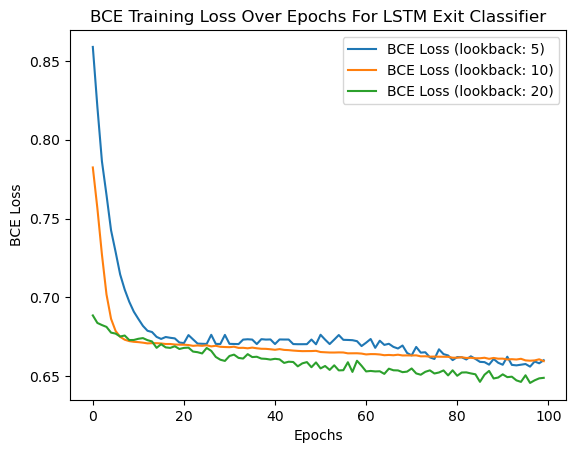
\includegraphics[width=0.5\textwidth]{training_loss.png} 
    \caption{Training Loss Curves for LSTM Model}
    \label{fig:example}
\end{figure}

\begin{figure}[H]
    \centering
    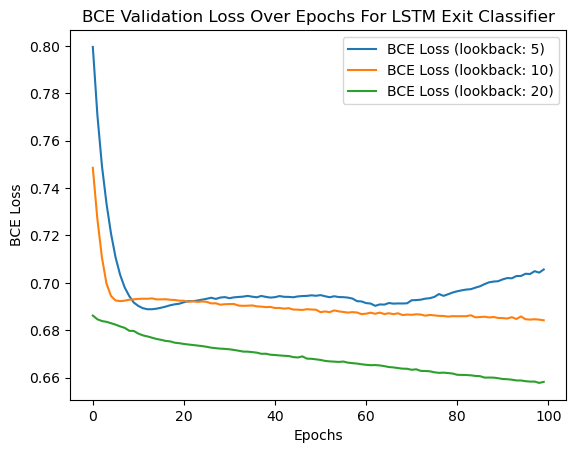
\includegraphics[width=0.5\textwidth]{validation_loss.png} 
    \caption{Validation Loss Curves for LSTM Model}
    \label{fig:example}
\end{figure}

\begin{figure}[H]
    \centering
    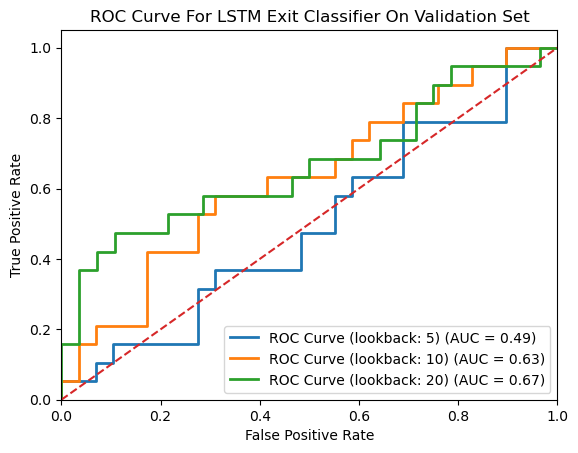
\includegraphics[width=0.5\textwidth]{roc_curve.png} 
    \caption{ROC Curves for LSTM Model}
    \label{fig:example}
\end{figure}

\begin{figure}[H]
    \centering
    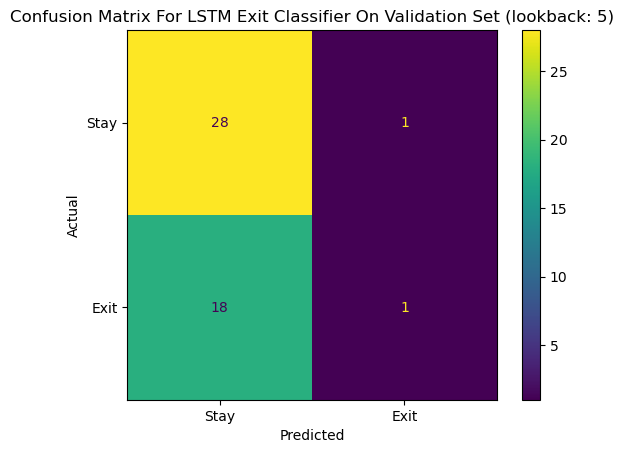
\includegraphics[width=0.5\textwidth]{conf_matrix1.png} 
    \caption{Confusion Matrix for LSTM Model With Lookback of 5}
    \label{fig:example}
\end{figure}

\begin{figure}[H]
    \centering
    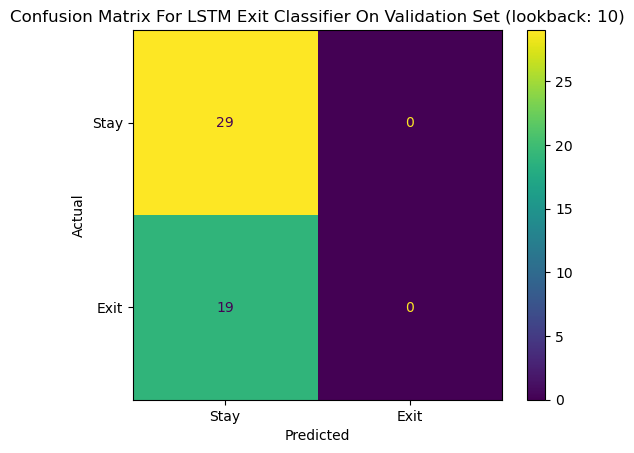
\includegraphics[width=0.5\textwidth]{conf_matrix2.png} 
    \caption{Confusion Matrix for LSTM Model With Lookback of 10}
    \label{fig:example}
\end{figure}

\begin{figure}[H]
    \centering
    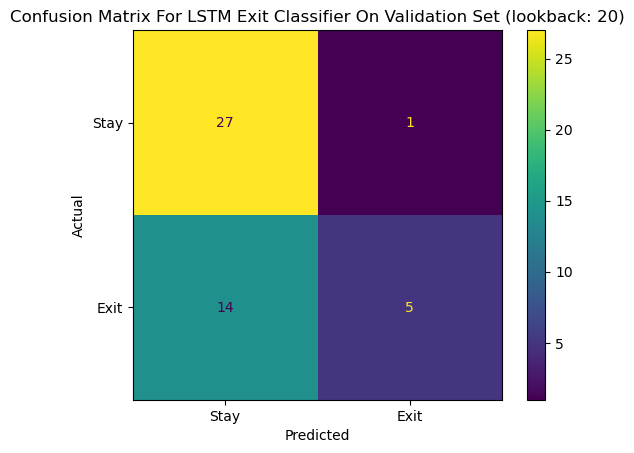
\includegraphics[width=0.5\textwidth]{conf_matrix3.png} 
    \caption{Confusion Matrix for LSTM Model With Lookback of 20}
    \label{fig:example}
\end{figure}

\newpage
\appendix

\section{Appendix A}
Please visit the \href{https://github.com/hrudhai98/vip-codebase}{GitHub} to view code. 




\bibliographystyle{apalike} % We choose the "plain" reference style
\bibliography{custom} % Entries are in the refs.bib file
\nocite{*}

 

\end{document}
